\documentclass[draft,linenumbers]{agujournal}
\draftfalse
\usepackage{hyperref}
\usepackage[export]{adjustbox}
\addtolength{\oddsidemargin}{-.875in}
\addtolength{\evensidemargin}{-.875in}
	
\hypersetup{
    colorlinks=true,
    linkcolor=blue,
    filecolor=magenta,      
    urlcolor=cyan,
}

\journalname{Journal of Advances in Modeling Earth Systems (JAMES)}

\begin{document}

\title{Supplementary Infomation for \emph{Parameteric controls on vegetation responses to biogeochemical forcing in the CLM5} by Fisher et al. (submitted to JAMES)}

    \begin{figure}[h]
     \centering
     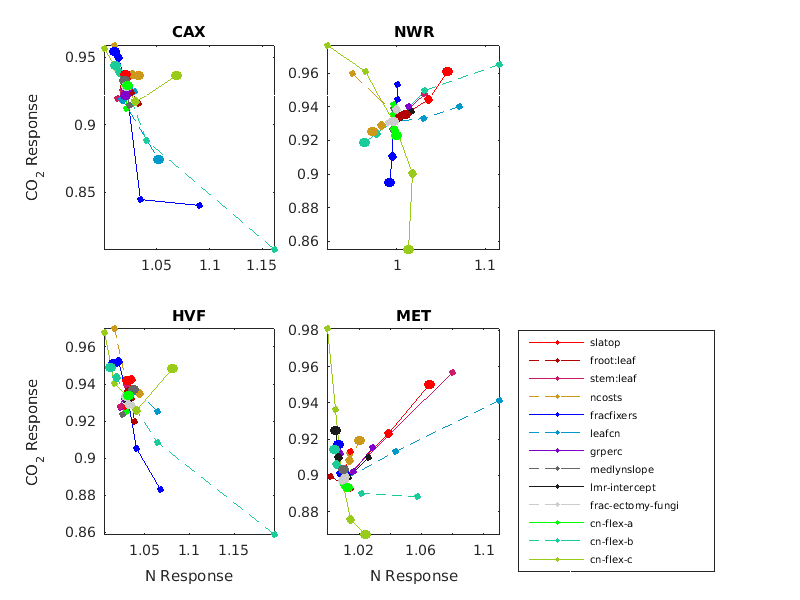
\includegraphics[width=1.55\textwidth, left]{matlab/figures/NOVc_CNdep_LEAFN1__p2012.png}
     \caption{Influence of parametric variation on the model response (fertilized/control) to 15 years of CO$_{2}$ and N fertilization on leaf nitrogen content ($N_{area}$), across the Caxiuan\~a (CAX), Niwot Ridge (NWR), Harvard Forest (HVF) and Metolious MET) sites.}
     \label{Leaf N CO2 and N respones 2001}
  \end{figure}
  
    \begin{figure}[h]
     \centering
     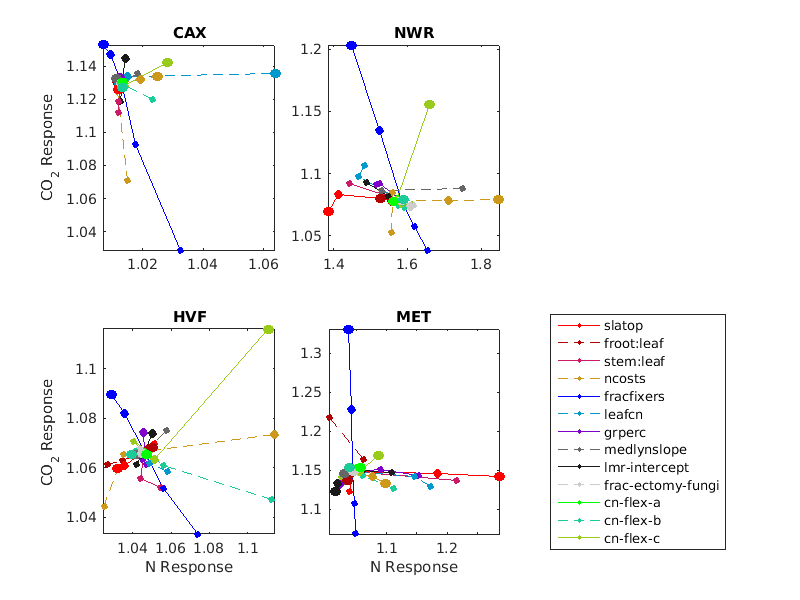
\includegraphics[width=1.55\textwidth, left]{matlab/figures/NOVc_CNdep_TOTVEGC1__p2012.png}
     \caption{Influence of parametric variation on the model response (fertilized/control) to 15 years of CO$_{2}$ and N fertilization on vegetation carbon, across the Caxiuan\~a (CAX), Niwot Ridge (NWR), Harvard Forest (HVF) and Metolious MET) sites.}
     \label{VEGC CO2 and N respones 2001}
  \end{figure}
  
\begin{figure}[h]
     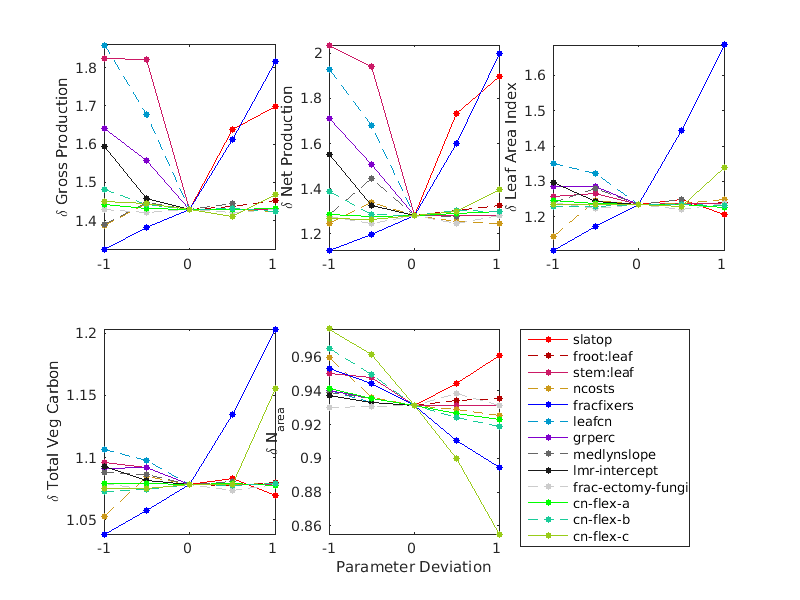
\includegraphics[width=1.2\textwidth]{matlab/figures/NOVc_FERT_1CLM50defpft_celev_1x1pt_US-NR1_ens_MIC_p1_2012.png}
     \caption{Influence of parametric variation (over the range tested: -1 to +1, Table \ref{table_ranges}) on the model response (fertilized/control) to 15 years of CO$_{2}$ fertilization (550ppm) at Niwot Ridge}
     \label{NR1 celev}
  \end{figure}
 
  \begin{figure}[h]
     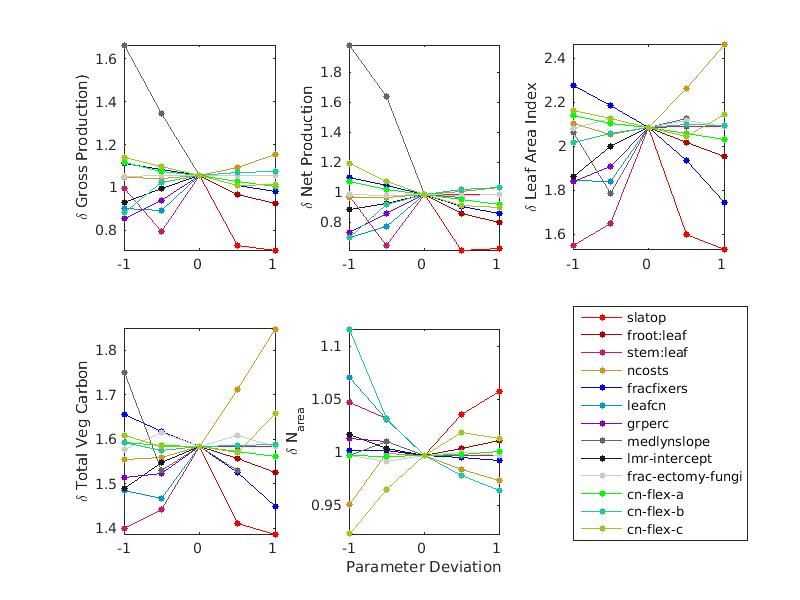
\includegraphics[width=1.2\textwidth]{matlab/figures/NOVc_FERT_1CLM50defpft_ndep_1x1pt_US-NR1_ens_MIC_p1.png}
     \caption{Influence of parametric variation (over the range tested: -1 to +1, Table \ref{table_ranges}) on the model response (fertilized/control) to 15 years of Nitrogen fertilization (+5 kgN m$^{2}$ y$^{-1}$) at Niwot Ridge}
     \label{NR1 ndep}
  \end{figure}
 

 \begin{figure}[h]
    % \centering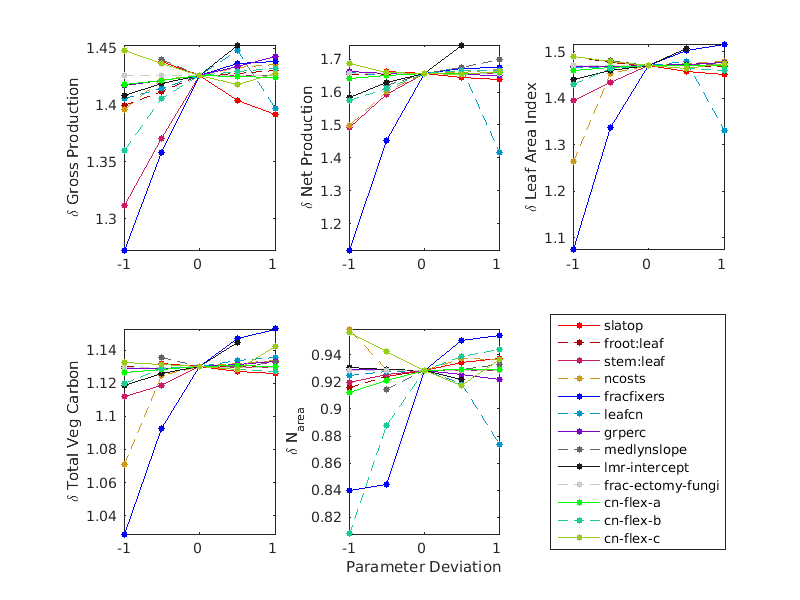
\includegraphics[width=0.5\textwidth, right]{lion-lo9
     \includegraphics[width=1.3\textwidth, left]{matlab/figures/NOVc_FERT_1CLM50defpft_celev_1x1pt_Br-cax_ens_MIC_p1_2012.png}
     \caption{Influence of parametric variation (over the range tested: -1 to +1) on the model response (fertilized/control) to 15 years of CO$_{2}$ fertilization (550ppm) at Caxiuan\~a }
     \label{CAX celev}
  \end{figure}

 \begin{figure}[h]
    % \centering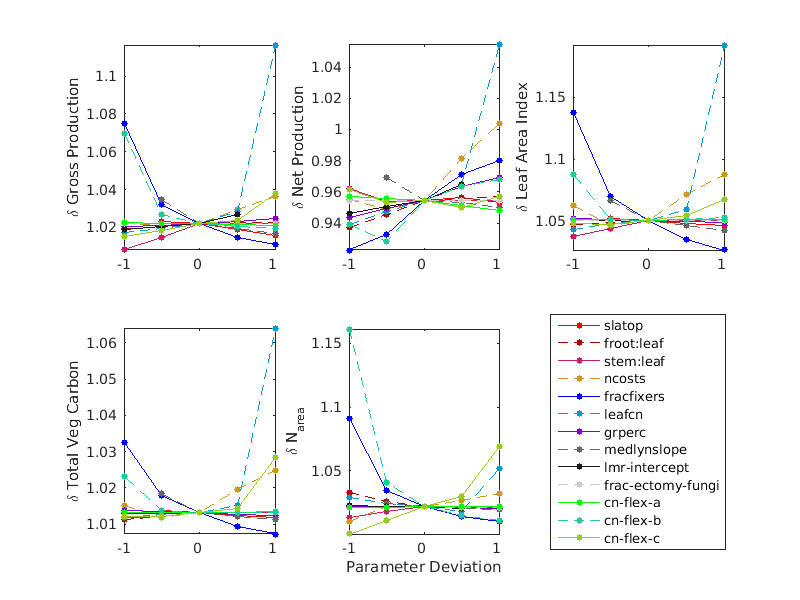
\includegraphics[width=0.5\textwidth, right]{lion-lo9
     \includegraphics[width=1.3\textwidth, left]{matlab/figures/NOVc_FERT_1CLM50defpft_ndep_1x1pt_Br-cax_ens_MIC_p1_2012.png}
     \caption{Influence of parametric variation (over the range tested: -1 to +1) on the model response (fertilized/control) to 15 uears of Nitrogen fertilization (+5 kgN m$^{2}$ y$^{-1}$) at Caxiuan\~a}
     \label{CAX ndep}
  \end{figure}
  
  \begin{figure}[h]
    % \centering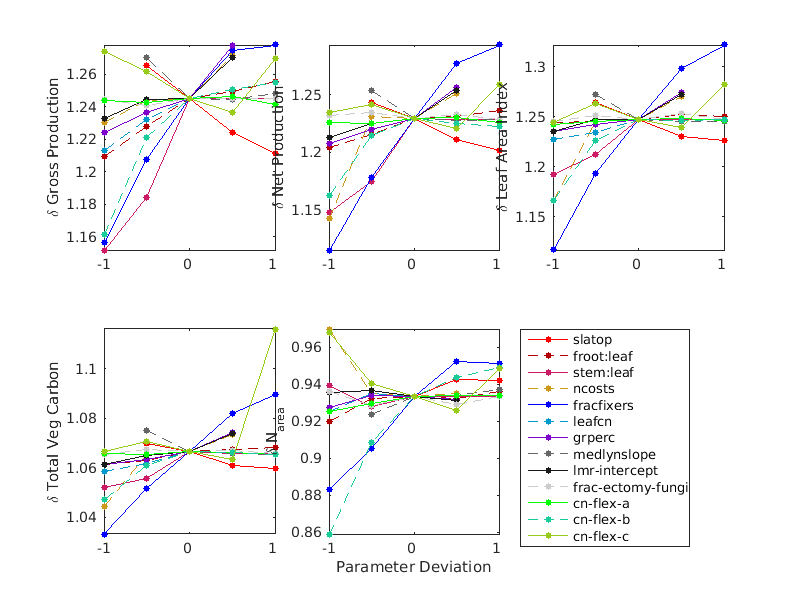
\includegraphics[width=0.5\textwidth, right]{lion-lo9
     \includegraphics[width=1.3\textwidth, left]{matlab/figures/NOVc_FERT_1CLM50defpft_celev_1x1pt_US_Ha1_ens_MIC_p1_2012.png}
     \caption{Influence of parametric variation (over the range tested: -1 to +1) on the model response (fertilized/control) to 15 years of CO$_{2}$ fertilization (550ppm) at Harvard Forest}
     \label{HRV celev}
  \end{figure}
  
  \begin{figure}[h]
    % \centering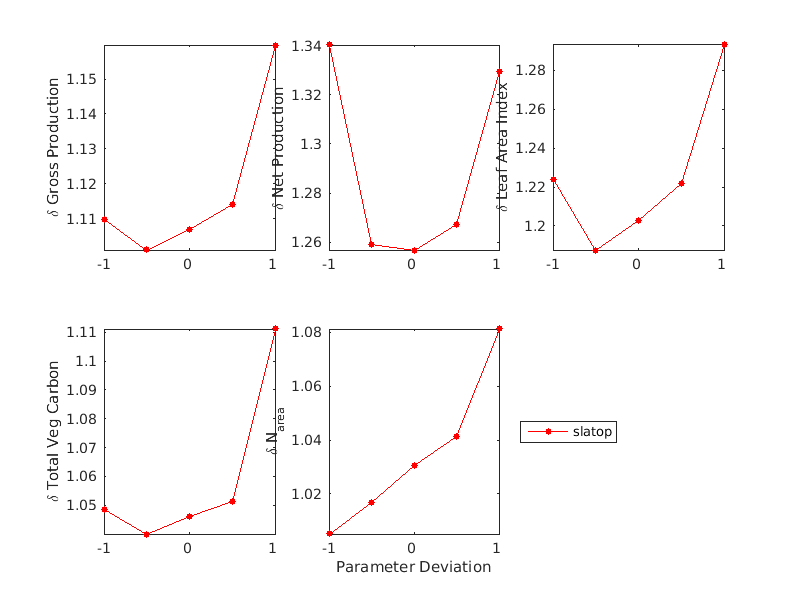
\includegraphics[width=0.5\textwidth, right]{lion-lo9
     \includegraphics[width=1.3\textwidth, left]{matlab/figures/NOVc_FERT_1CLM50defpft_ndep_1x1pt_US_Ha1_ens_MIC_p1_2012.png}
     \caption{Influence of parametric variation (over the range tested: -1 to +1) on the model response (fertilized/control) to 15 years of Nitrogen fertilization (+5 kgN m$^{2}$ y$^{-1}$) at Harvard Forest}
     \label{HRV ndep}
  \end{figure}
  
  \begin{figure}[h]
    % \centering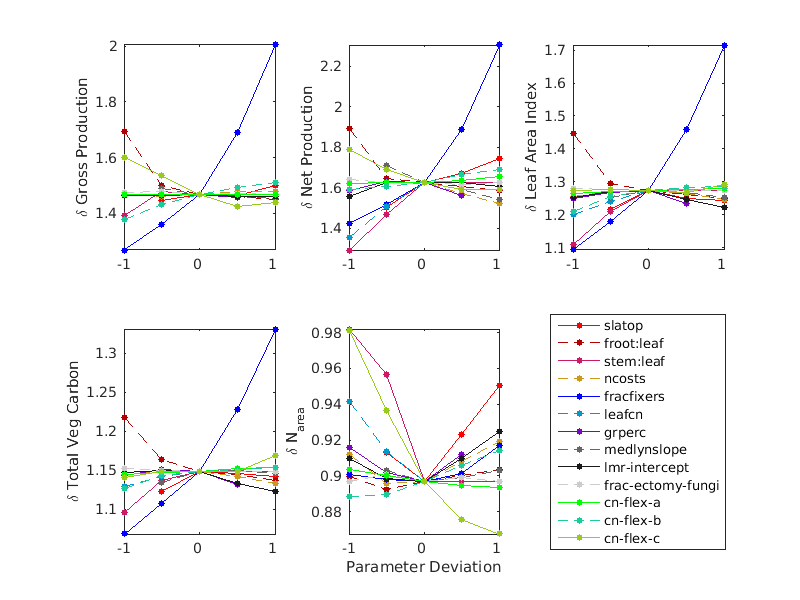
\includegraphics[width=0.5\textwidth, right]{lion-lo9
     \includegraphics[width=1.3\textwidth, left]{matlab/figures/NOVc_FERT_1CLM50defpft_celev_1x1pt_US-Me2_ens_MIC_p1_2012.png}
     \caption{Influence of parametric variation (over the range tested: -1 to +1) on the model response (fertilized/control) to 15 years of CO$_{2}$ fertilization (550ppm) at Metolius Forest}
     \label{MET celev}
  \end{figure}
  
  \begin{figure}[h]
    % \centering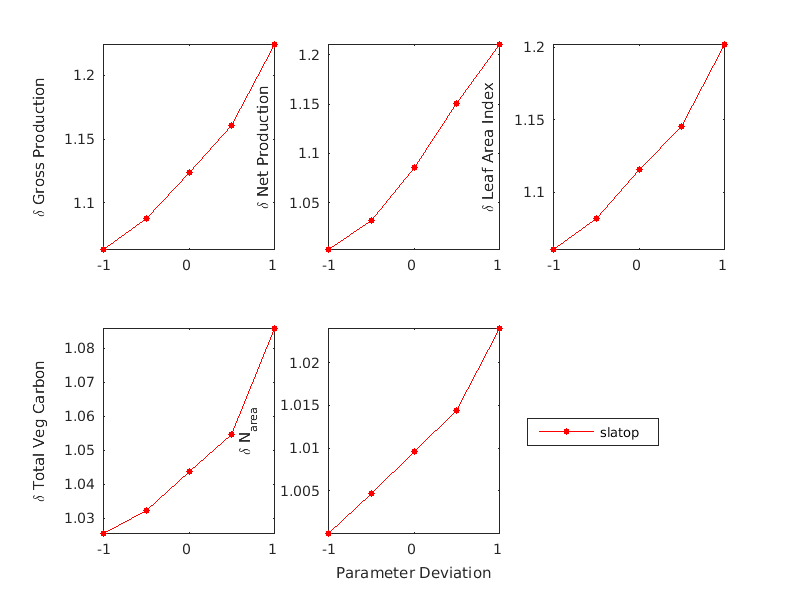
\includegraphics[width=0.5\textwidth, right]{lion-lo9
     \includegraphics[width=1.3\textwidth,left]{matlab/figures/NOVc_FERT_1CLM50defpft_ndep_1x1pt_US-Me2_ens_MIC_p1_2012.png}
     \caption{Influence of parametric variation (over the range tested: -1 to +1) on the model response (fertilized/control) to 15 years of Nitrogen fertilization (+5 kgN m$^{2}$ y$^{-1}$) at Metolius Forest}
     \label{MET ndep}
  \end{figure}
  


\end{document}